\documentclass{beamer}

\usepackage{lmodern}
\usepackage[utf8]{inputenc}
\usepackage[T1]{fontenc}
\usepackage[french]{babel}
\usepackage{url}
\usepackage{listings}

\graphicspath{ {../doc/img/} }

\usetheme{Madrid}
\usecolortheme{default}

\title[Analyse de données d'eye-tracking]{Analyse de données d'eye-tracking}
\subtitle{Présentation du TER}
\author[STAVRIDIS Adonis]{STAVRIDIS Adonis}
\institute[Unistra, iCube]{
  Université de Strasbourg \and iCube
}
\date[TER]{26 Mai 2021}

\begin{document}

%-------------------------------------------------------------------------------
\frame{\titlepage}
%-------------------------------------------------------------------------------
\begin{frame}
  \frametitle{Introduction}

  \begin{block}{Eye-tracking / Oculométrie}
    technologie qui permet de reconnaître la position du regard d’un individu
    dans un environnement réel ou virtuel
  \end{block}
  \pause
  \begin{figure}
    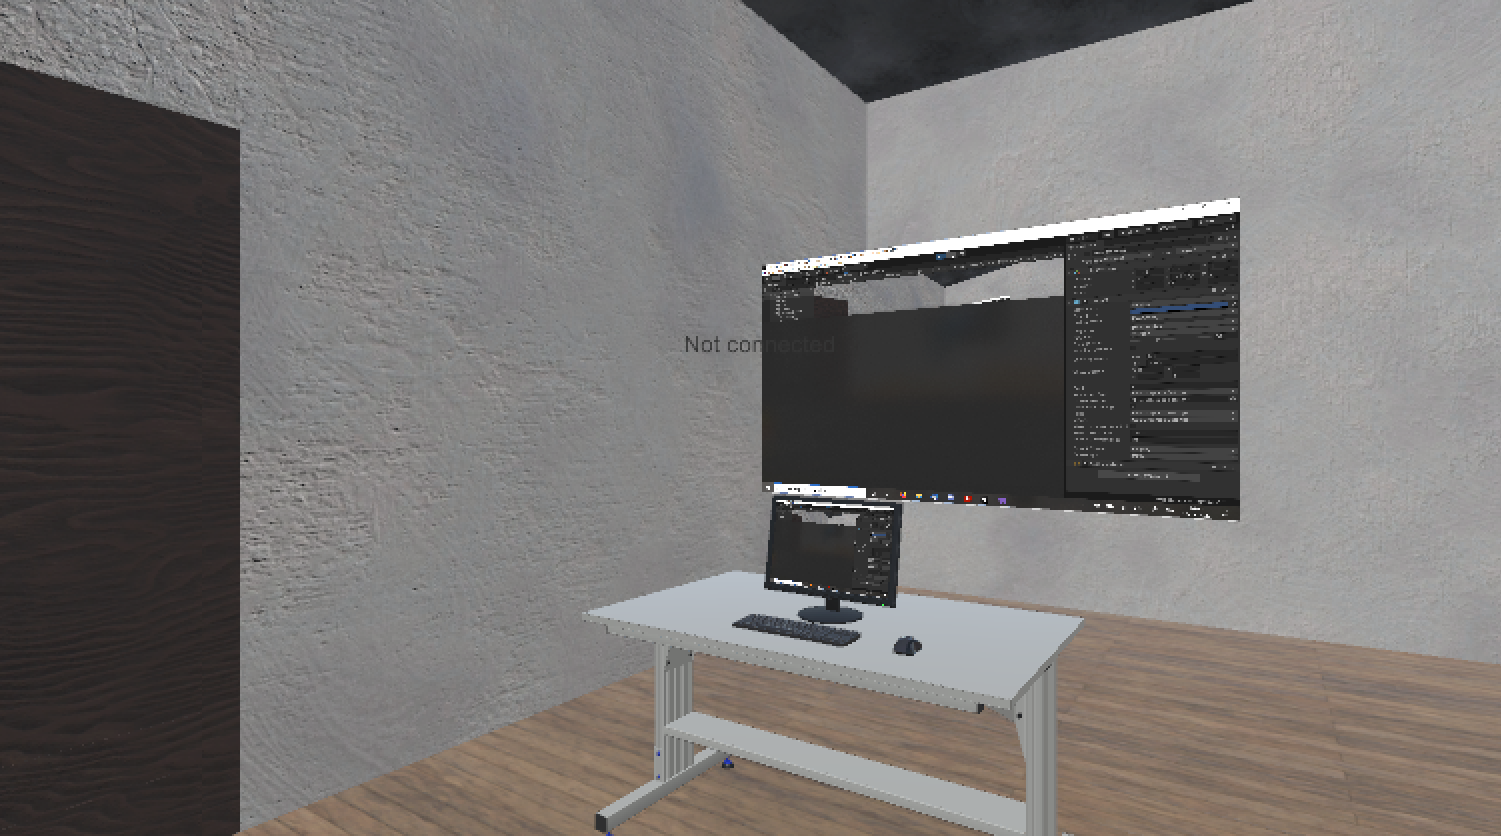
\includegraphics[height=0.35\textwidth]{environnement.png}
    \caption{Environnement de travail virtuel}
  \end{figure}
\end{frame}
%-------------------------------------------------------------------------------
\begin{frame}
  \frametitle{Sommaire}

  \tableofcontents
\end{frame}
%-------------------------------------------------------------------------------
\section{Capteurs}
%-------------------------------------------------------------------------------
\begin{frame}
  \frametitle{Capteurs}

  \begin{columns}
    \column{0.5\textwidth}
    \begin{figure}
      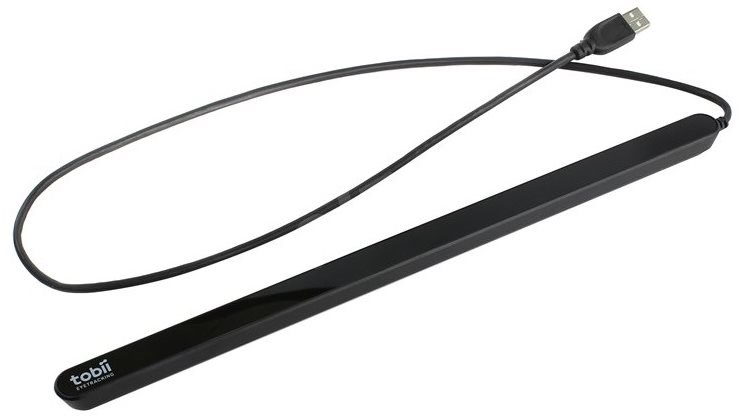
\includegraphics[height=0.35\textwidth]{tobii.jpeg}
      \caption{Capteur d'écran Tobii}
    \end{figure}
    \column{0.5\textwidth}
    \begin{figure}
      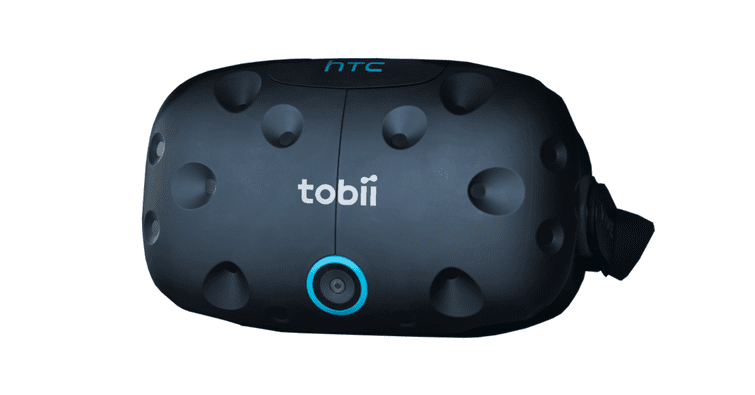
\includegraphics[height=0.35\textwidth]{htcvive.png}
      \caption{Casque de réalité virtuelle avec capteurs intégrés}
    \end{figure}
  \end{columns}
\end{frame}
%-------------------------------------------------------------------------------
\section{Analyse des données}
%-------------------------------------------------------------------------------
\begin{frame}[fragile]
  \frametitle{Analyse des données}
  \begin{lstlisting}
    <temps> : <positionX>, <positionY>
    0.00 : 50, 50
    0.25 : 43, 64
    0.50 : 38, 75
    0.75 : 41, 66
    ...
  \end{lstlisting}
\end{frame}
%-------------------------------------------------------------------------------
\begin{frame}
  \frametitle{Analyse des données}
  \begin{figure}
    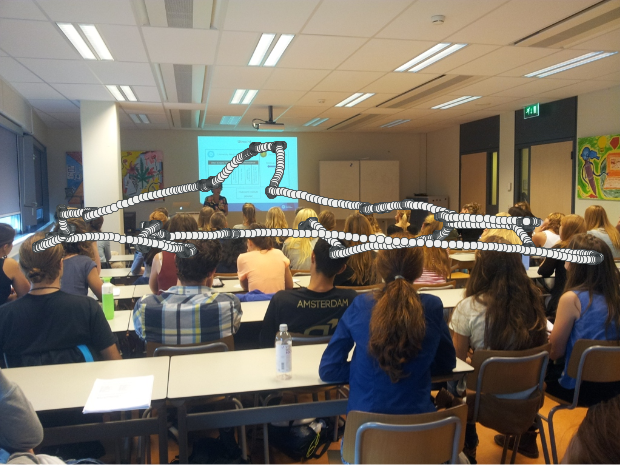
\includegraphics[height=0.5\textwidth]{raw.png}
    \caption{Positions des fixations}
  \end{figure}
\end{frame}
%-------------------------------------------------------------------------------
\begin{frame}
  \frametitle{Analyse des données}
  \begin{figure}
    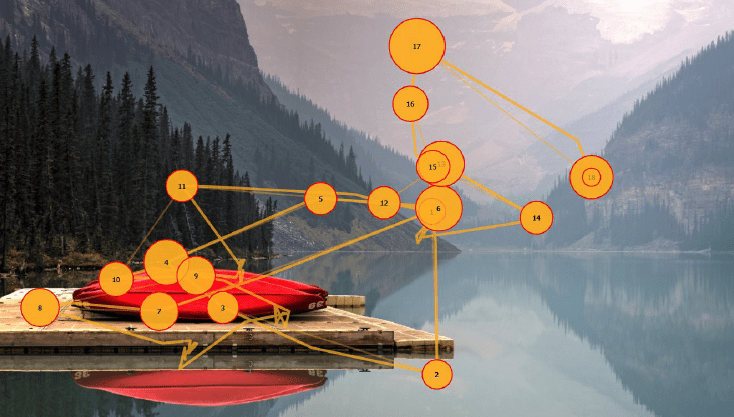
\includegraphics[height=0.5\textwidth]{sequence.png}
    \caption{Séquence de fixations}
  \end{figure}
\end{frame}
%-------------------------------------------------------------------------------
\begin{frame}
  \frametitle{Analyse des données}
  \begin{figure}
    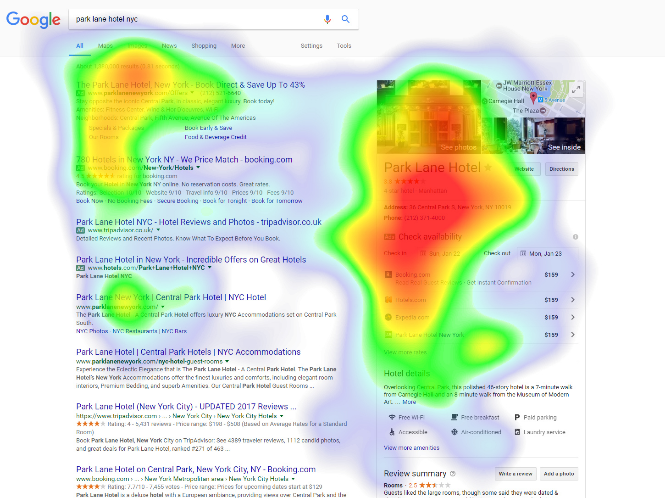
\includegraphics[height=0.5\textwidth]{heatmap.png}
    \caption{Carte de chaleur}
  \end{figure}
\end{frame}
%-------------------------------------------------------------------------------
\section{Implémentation}
%-------------------------------------------------------------------------------
\section{Résultats}
%-------------------------------------------------------------------------------
%Example of the \pause command
\begin{frame}
  In this slide \pause

  the text will be partially visible \pause

  And finally everything will be there
\end{frame}
%-------------------------------------------------------------------------------
%Highlighting text
\begin{frame}
  \frametitle{Sample frame title}

  In this slide, some important text will be
  \alert{highlighted} because it's important.
  Please, don't abuse it.

  \begin{block}{Remark}
    Sample text
  \end{block}

  \begin{alertblock}{Important theorem}
    Sample text in red box
  \end{alertblock}

  \begin{examples}
    Sample text in green box. The title of the block is ``Examples".
  \end{examples}
\end{frame}
%-------------------------------------------------------------------------------


%-------------------------------------------------------------------------------
%Two columns
\begin{frame}
  \frametitle{Two-column slide}

  \begin{columns}

    \column{0.5\textwidth}
    This is a text in first column.
    $$E=mc^2$$
    \begin{itemize}
      \item First item
      \item Second item
    \end{itemize}

    \column{0.5\textwidth}
    This text will be in the second column
    and on a second tought this is a nice looking
    layout in some cases.
  \end{columns}
\end{frame}
%-------------------------------------------------------------------------------


\end{document}
